\documentclass[10pt,twocolumn,letterpaper]{article}

\usepackage{cvpr}
\usepackage{times}
\usepackage{epsfig}
\usepackage{graphicx}
\usepackage{amsmath}
\usepackage{amssymb}
\usepackage{hyperref}
\usepackage{booktabs}
\usepackage{subcaption}
\usepackage{comment}
\usepackage{multirow}


% Include other packages here, before hyperref.

% If you comment hyperref and then uncomment it, you should delete
% egpaper.aux before re-running latex.  (Or just hit 'q' on the first latex
% run, let it finish, and you should be clear).
\usepackage[breaklinks=true,bookmarks=false]{hyperref}

\cvprfinalcopy % *** Uncomment this line for the final submission

\def\cvprPaperID{****} % *** Enter the CVPR Paper ID here
\def\httilde{\mbox{\tt\raisebox{-.5ex}{\symbol{126}}}}

% Pages are numbered in submission mode, and unnumbered in camera-ready
%\ifcvprfinal\pagestyle{empty}\fi
\setcounter{page}{1}
\begin{document}

%%%%%%%%% TITLE
\title{Face mask detector: a Computer Vision application}

\author{Federico Agostini\\
{\tt\small federico.agostini.5@studenti.unipd.it }
% For a paper whose authors are all at the same institution,
% omit the following lines up until the closing ``}''.
% Additional authors and addresses can be added with ``\and'',
% just like the second author.
% To save space, use either the email address or home page, not both
\and
Federico Bottaro\\
{\tt\small federico.bottaro.1@studenti.unipd.it}
}

\maketitle
%\thispagestyle{empty}

%%%%%%%%% ABSTRACT
\begin{abstract}
The very recent Covid-19 outbrake forced the population to adopt new habits in order to prevent and control the spreading of the disease. In particular, face masks represent one of the most important means to reduce its advance. Computer Vision and Neural Networks can be exploited to ensue the respect of these new social rules. The aim of this work is to build a pipeline to detect and recognize whether people are wearing face masks, both in images, in videos and in real time. The results of this work can be applied to automate the surveillance in public places, where human control can be a difficult task.

%In the very recent period Computer Vision is a fundamental subject for fighting the Covid-19. In this document we are going to see an application regarding the face mask recognition. In particular we want to classify images of people wearing or not a mask. The aim of this work is exploiting some Computer Vision's tools to recognize faces and analyze the frame using several types of neural networks to be able to have a classification also in a non trivial scenarios.
\end{abstract}

%%%%%%%%%%%%%%%%%%%%%%%%%%%%%%%%%%%%%%%%%%%%%%%%%%%%%%%%%%%%%%%%%%%%%%%%%%%%%%%%%%%%%%%%%%%%%%%%%%
%%%%%%%%%%%%%%%%%%%%%%%%%%%%%%%%%%%%%%%%%%%%%%%%%%%%%%%%%%%%%%%%%%%%%%%%%%%%%%%%%%%%%%%%%%%%%%%%%%
%%%%%%%%%%%%%%%%%%%%%%%%%%%%%%%%%%%%%%%%%%%%%%%%%%%%%%%%%%%%%%%%%%%%%%%%%%%%%%%%%%%%%%%%%%%%%%%%%%

%%%%%%%%% BODY TEXT
\section{Introduction}
\label{sec:introduction}
Covid-19 epidemic highlighted the usage of face masks as the primary mean to contain and reduce the spreading of the disease. Many Countries decided to make it mandatory in public and crowded places. However, acting a strong control could be a difficult task for the Governments and Police forces without the use of Artificial Intelligence (AI). AI along with Computer Vision (CV) can be exploited to enhance and automate the process of controlling the respect of these basic social rules.

This work aims to build an autonomous system that can detect whether people wear face masks. The task can be split in two different ones(as suggested in~\cite{PyImage}):
\begin{itemize}
    \item Build and train a Neural Network (NN) to understand whether a person is wearing or not the face mask from an image of the face;
    \item Apply a face detector to extract faces from images and video, and then process them using the NN developed in the previous step.
\end{itemize}

The learning paradigm adopted to train the NN is supervised learning; hence we used a labelled dataset to build the classificator, which is discussed in Section~\ref{sec:data}. The final performances will be influenced by the complexity of the data, and the actual scenarios where the NN should be applied also will depend on it. The architecture and the implementation of both the NN and the face detector, that is implemented throght the CV package \texttt{OpenCV}, are developed in Section~\ref{sec:methods}.

\begin{comment}
In the last few months the Covid-19 disease has spread throughout the entire world. One of the most powerful method to reduce spreading is the use of the face mask. A lot of countries move in this direction making the use of the face mask mandatory in public. Due to the power and the variety of the symptomatology of the disease, acting a strong control is a difficult task for the governments and their police forces. The development of subjects such as computer vision (CV) and artificial intelligence (AI) can be exploited to act a control strategy on the use of this fundamental self protection method. \\Our work consists in combining different aspect of CV and AI to analyze the behavior of peoples, in particular we want to recognize the use of the face mask. To achieve this task we focused on using neural networks (NN) as a prediction model. We use different types of NNs to make the classification but all the models shares the same learning paradigm: supervised learning (meaning that there are some label associate to each data).\\First of all we search some dataset with a sufficient large number of images to be able to train a network, the second chapter of the document explore in the details the different type of data we used. Once the data was collected we split our work in two main topic:

\begin{itemize}
    \item Search a NN structure to be able to predict if a given person are wearing a face mask or not.
    \item Explore the field of face detectors to be able to recognize faces also in a non trivial image with the scope of passing single faces to the prediction's environment to find out who is wearing a mask.
\end{itemize}

 As we can understand the schedule is very simple but the combination of AI with CV is necessary: NNs are one of the best prediction model existing nowadays but to act in a real life scenario the use of CV is mandatory. If we think for example to a camera looking for a public square, there is the necessity to distinguish faces from all the other objects to be able to pass only the desired information 
to the predictor in order to obtain a good performance. 
\end{comment}

%%%%%%%%%%%%%%%%%%%%%%%%%%%%%%%%%%%%%%%%%%%%%%%%%%%%%%%%%%%%%%%%%%%%%%%%%%%%%%%%%%%%%%%%%%%%%%%%%%
%%%%%%%%%%%%%%%%%%%%%%%%%%%%%%%%%%%%%%%%%%%%%%%%%%%%%%%%%%%%%%%%%%%%%%%%%%%%%%%%%%%%%%%%%%%%%%%%%%
%%%%%%%%%%%%%%%%%%%%%%%%%%%%%%%%%%%%%%%%%%%%%%%%%%%%%%%%%%%%%%%%%%%%%%%%%%%%%%%%%%%%%%%%%%%%%%%%%%

\section{Dataset}
\label{sec:data}
The quality of the dataset used to train the NN heavily influences its performance in real life scenarios. Since the novelty of the task, there are no big and well established labelled datasets of people wearing face masks. One possible solution (suggested in the work of Prajna Bhandary~\cite{Prajna}) is to artificially build our data by placing images of face masks on top of existing face pictures, using facial landmarks to put it in the right position. The drawback of this approach is that it could lack of generalization capabilities, and not perform well when applied in different situations. In addition, it may only learn to identify masks with the same color as the one used to build the dataset, whether they can have different shapes and colors.

\begin{figure}[htp]
    \centering
    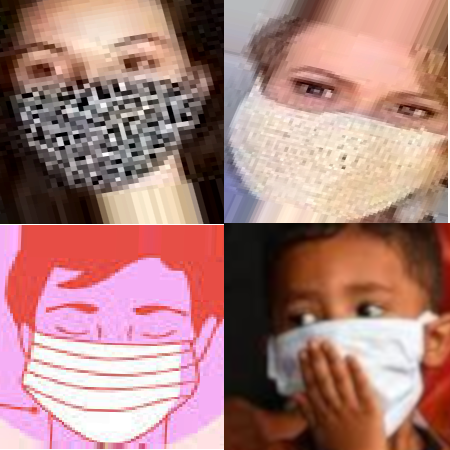
\includegraphics[width=0.50\linewidth]{Tex_proj/figure/4face.png}
    \caption{Examples of images used to train the network.}
    \label{fig:ex_fig_2}
\end{figure}

The dataset we decided to use is hosted on \textit{Kaggle}~\footnote{\href{https://www.kaggle.com/ashishjangra27/face-mask-12k-images-dataset}{https://www.kaggle.com/ashishjangra27/face-mask-12k-images-dataset}.}. This one combines both real and stylized images, as shown in Fiure~\ref{fig:ex_fig_2}. The original dataset is split into training, validation and test subsets; however we decided to join train and validation, in order to increase the size of the training set. Even in this way, the number of images of people wearing face masks is quite small (about 800); to overcome this problem, data augmentation is performed stretching, rotating and performing random crop (see Figure~\ref{fig:ex_aug_5}). One weakness of the data resides in the fact that all the images are more or less frontal picture, so we can loose accuracy in prediction when dealing with different perspectives.

\begin{figure}[htp]
    \centering
    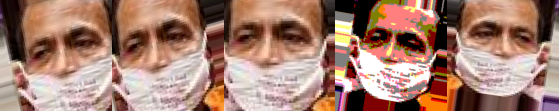
\includegraphics[width=0.99\linewidth]{Tex_proj/figure/augmentation.pdf}
    \caption{Examples of augmentation in train data with mask.}
    \label{fig:ex_aug_5}
\end{figure}

At the end our dataset is composed by:
\begin{itemize}
    \item \textbf{Training set}:
    \begin{itemize}
        \item 4011 with mask (815 originals + 3196 augmented)   \item 5401 without mask
    \end{itemize}
    \item \textbf{Test set}:
    \begin{itemize}
        \item 483 with mask
        \item 509 without mask
    \end{itemize} 
\end{itemize}

The dataset described above is used to train the NN; in addition, the complete algorithm (face detector + face mask discriminator) is tested over some images and videos acquired from the web.

%The research  of a good dataset to explore field such as CV may seems an easy task and often this task is omitted from reports. In reality without a good structure of the dataset is impossible to train our environment. In our specific task we need not only some images of people wearing a mask or not but due to the fact that we choose a supervised learning paradigm we have to look for a labelled data. So the first choice is to build in a simple way our dataset with the label. Fallowing the work of Prajna Bhandary ~\cite{Prajna} we search in the web for some images of faces without mask and in this case we can choose a dataset also without any description; then we add two different \textit{.png} stylized images representing a face mask. The problem with this approach is the flexibility of the learning. In fact having all times the same two mask we have an high risk of overfitting over these pictures driving as to a bad prediction model that can understand the use of a face mask only if the face mask is really similar to one of the two proposed.\\This approach can be good because in the web there isn't a good quantity of images with people wearing a face mask due to the fact that the use in large scale of this tool is really recent. With a little bit of more investigation and to the light of the problem with the first approach, we found a dataset from \textit{Kaggle.com}~\footnote{\href{https://www.kaggle.com/ashishjangra27/face-mask-12k-images-dataset}{Dataset link}.}.\\ This dataset is composed by very different type of images for bot the category (with and without mask), we have for example some real faces centered in the picture or some highly stylized images. We can see some examples in figure \ref{fig:ex_fig_2}. 

%As is possible to see from the link in the footnotes we have that the dataset is split in three different categories: train, validation and test set. We reorganize our data in only two category merging the validation and the train in order to obtain a new train set and the old test set. Also with this configuration we have a dataset poor in number of images with mask (images without mask are not difficult to find) in fact we are currently dealing with about 800 images. To improve the number of the training set with mask we use a data augmentation technique. Starting from a single image we stretch and rotate the original one and we save several new modified copies. Also the RGB channel is modified sometimes as we can see in figure \ref{fig:ex_aug_5}

%As we will present later in the code section another modification of the images is performed, in particular we modify the shape of the picture to pass it to the NNs and a RGB mean subtraction is needed for the face detector due the learning technique adopted.\\ For the test we explore various type of data. First of all we test our algorithm of the test set given with the train; then we change the input of our network in order to analyze some video and also in a streaming set up, catching the video directly from the PC cam  and processing in real time the information. For this two last implementation we "build" our dataset making some videos to ourself. 

%%%%%%%%%%%%%%%%%%%%%%%%%%%%%%%%%%%%%%%%%%%%%%%%%%%%%%%%%%%%%%%%%%%%%%%%%%%%%%%%%%%%%%%%%%%%%%%%%%
%%%%%%%%%%%%%%%%%%%%%%%%%%%%%%%%%%%%%%%%%%%%%%%%%%%%%%%%%%%%%%%%%%%%%%%%%%%%%%%%%%%%%%%%%%%%%%%%%%
%%%%%%%%%%%%%%%%%%%%%%%%%%%%%%%%%%%%%%%%%%%%%%%%%%%%%%%%%%%%%%%%%%%%%%%%%%%%%%%%%%%%%%%%%%%%%%%%%%

\section{Method}
\label{sec:methods}
%We can now go a little bit deeper in our task starting to discuss the method that we choose for solve the problem of the face mask recognition. To attach this challenge we choose to split the problem in two:
As introduced in Section~\ref{sec:introduction}, our approach implies to split the problem in two tasks:
\begin{itemize}
    %\item Given a picture of a face, that are more or less centered in the image, we want to make the binary classification of the mask use.
    \item Train and use a binary NN classificator, which can identify whether a face mask is used given a picture of a person's face;
    %\item Given a picture with one or more peoples, in a daylife situation, we want to extract the areas of our interest (that are the faces) to be able to give a uniform input to the predictor.
    \item Extract Regions of Interest (ROIs) from generic images and then process them through the classifier. In our scenario, ROIs are represented by faces, so a face detector is implemented. 
\end{itemize}

To tackle the first point, two solutions are proposed. First of all, a simple model with a convolutional architecture is built from scratch and trained over our dataset; in addition, also a transfer learning approach is tested. In this second case, a pretrained Network is adopted as base model, which was trained over a large dataset, and on top of that a fully connected part is constructed: in this way the abstract feature learned by the base model are exploited to solve our specific classification.

The face detection instead is carried out by taking advantage of a pretrained model available in the OpenCV library.

%In general we have that to reach great performances in a recognition task is needed to have a complex system and a powerful hardware to train the Networks according to the complexity and the variety of the object that we can interface with. To solve this problem we decide to adopt a transfer learning technique. In particular we can adapt some pre existing Neural Networks that are already trained in some very big dataset with different features by keeping fixed the weight of the layer away from the end of the NN. In doing this we are not touching the abstract feature of the learning and we need to train only the last layers to obtain significative information.

\subsection{Simple Convolutional NN}
\label{NN_1}
The classification model is built using \texttt{Keras}~\cite{keras} that is a frontend for Tensorflow, a machine learning environment developed by Google. Figure~\ref{fig:grafo} describes the architecture of the Network. It is composed by three convolutional layers alternated by MaxPooling ones, while the final part flattens the result and propagates it through three fully connected layers; moreover, dropout is implemented both in the convolutional and in the fully connected section, in order to add some regularization during the learning phase. The last neuron features a Sigmoid activation function to perform the binary classification: in this way it is also possible to extract a probability estimate of the prediction. From now we refer to this model as \textit{Convolutional Network}.

%With this environment we try to build our own simple neural network before exploring the field of transfer learning. In particular we use a model with a combination of various type of layer Figure \ref{ig:grafo} in Appendix  is a schematic representation of our Network drawn by Keras. As we can see we have some convolutional layer and we add as last layer a single neuron with a sigmoid activation function. In doing so we want to extract not only a binary classification but we are able also to give a quantitative goodness of the prediction. With this we mean that an output value closer to the extremes of the function guarantees a better classification accuracy with respect to an output in the middle. 

In addition to the preprocessing explained in Section~\ref{sec:data}, each image is resized to $224\times224$ pixels, and each RGB channel is normalized to 1. The appropriate loss for the task is the binary crossentropy, and the learning process is guided by the Adam optimizer; in addition, also a scheduler is implemented to control the learning rate in an exponential decreasing way. Training is carried out for 20 epoches, using batches of 128 images. 

Even with this simple structure, results show good performances; a more detailed and accurate description, along with the comparison with the transfer learning approach, is presented in Section~\ref{sec:results}.
%To train the model a standard procedure is performed, given as input the images with their respective label, an Adam optimizer is selected to reach the minimum if the loss function. Due to the nature of the classification we choose a binary cross entropy. To reduce the risk random jump when the loss approach the minimum we impose an adaptive learning rate and in particular an exponential decay provided by Keras is used. To have a results without the necessity of a strong hardware the train runs for 20 epochs. As we will see in the results section also with this simple structure we can reach good performances. The results that we obtain using this model will be presented in the next section with a comparison with the other infrastructure used.

\subsection{Transfer learning}
%As we will see in the results section, the network presented in section \ref{NN_1} reach a good accuracy (about 97\%).To improve this result we have to use a model with more complexity capable to understand more complex and deeper features of the proposed task. A state of the art engine of computer vision is MobileNetv2~\cite{s2018mobilenetv2} that is a very deep Network trained of ImageNet. ImageNet is a large dataset of picture containing a lot of different category of object. Due to the complexity of the training and the large amount of data we upload the weights of the network directly from Keras and we do not make a complete training of the network.\\ Our goal is make a binary classification so we have the necessity to modify the given Network, the work here can be split in two parts:

Transfer learning is a technique where a Network pre-trained over a large dataset is used as a base model in order to take advantage of its knowledge of low level features; on top of that another Network is built to achieve a specific task, in our case to recognize the presence or absence of a face mask.

MobileNetV2~\cite{s2018mobilenetv2} represents the state of the art architecture for mobile and resource constrained environments. In particular, it is trained over the ImageNet~\cite{imagenet_cvpr09} dataset. Due to the complexity of the architecture, and the huge amount of images in the dataset, training is infeasible without proper hardware: hence the weights are downloaded from \texttt{Keras} and the architecture freezed, so they are not updated.
The head model adapts MobileNetV2 to perform the binary classification task: an average pooling layer precedes two fully connected ones, with dropout. The final neuron activates with a Sigmoid function, as the previous convolutional model.

Learning is performed by the Adam optimizer, with an exponential decay scheduler. The duration is set to 20 epoches.

This solution is referred as \textit{MobileNetV2} in the next Sections.

\subsection{Face detector}
In a real application it is very difficult to have only one person that stands in front of a camera waiting for a response of the program. It is more likely to have a situation where different people are moving into a room or in a public square and so the frame catched by the camera is more complex with respect to the ones used to train the prediction network. In such scenario there are several strategies that may work; we decide to implement a CV method to recognize and extract faces in a given frame. 
%In particular, another pre-trained NN is exploited and again we adapt the output of that network in order to have a series of images representing the faces recognized, where present, in the given picture.
The Network used for this task is a Residual Network, in particular ResNet-10. This category of networks features "identity shortcut connections" that skips one or more layers. Network architecture and weights can be downloaded from \texttt{OpenCV} Github repository\footnote{\href{https://github.com/opencv/opencv/tree/master/samples/dnn/face_detector}{https://github.com/opencv/opencv/tree/master/samples/dnn/face\_detector}}. It is built with Caffe~\cite{jia2014caffe} and trained with the SSD framework~\cite{liu2016ssd} over the WIDER face dataset~\cite{yang2016wider}. The usage of a pre-trained Network is due to the fact that great hardware resources and time are required to train a good detector. In addition, it should be more accurate with respect to \texttt{OpenCV} Haar Cascade when analyzing faces with different viewing angles and not only on straight on perspective.

This face detector requires that input images are preprocessed by resizing them to $300\times300$ pixels and acting mean subtraction in each RGB channel. Given a frame, the output is composed by the list of objects detected (represented by left, top, right, bottom margin with coordinates represented as fraction of the whole image) plus a confidence value, that can be used to tune the sensibility of the prediction.\\

Summing up, the face detector extracts faces from the images, which become the input for our Network built with \texttt{Keras}, that will predict whether a mask is worn.

%We want now to summarize the work in few line before present the results. We use ResNet10 to extract faces from a given input (as we will see we try to explore not only the static pictures but we try to make some prediction also to some videos and related); then we use our convolutional network or MobileNetv2 to analyze the faces and make the prediction on the mask.

%%%%%%%%%%%%%%%%%%%%%%%%%%%%%%%%%%%%%%%%%%%%%%%%%%%%%%%%%%%%%%%%%%%%%%%%%%%%%%%%%%%%%%%%%%%%%%%%%%
%%%%%%%%%%%%%%%%%%%%%%%%%%%%%%%%%%%%%%%%%%%%%%%%%%%%%%%%%%%%%%%%%%%%%%%%%%%%%%%%%%%%%%%%%%%%%%%%%%
%%%%%%%%%%%%%%%%%%%%%%%%%%%%%%%%%%%%%%%%%%%%%%%%%%%%%%%%%%%%%%%%%%%%%%%%%%%%%%%%%%%%%%%%%%%%%%%%%%

\section{Experiments and results}
\label{sec:results}
%Once that all the methods are explained, we can move to the results obtained from our works.
%Starting from predictors, we want to make a comparison between the convolutional network and MobileNetv2. The idea behind the construction of our convolutional network is that we are dealing with a dataset with different type of face ans mask (as discussed in section \ref{data}) but all share the same category: they are more or less frontal pictures and so we can conclude that the dataset is not so hard to learn. On the other hand we have a very complex network that is pre trained model so only the last layer (added to get the classification on the mask) need to be trained and also in this case the task is not so difficult and do not require an high computational power.
\subsection{Neural Network classifier}
We start analyzing the results of the training for our convolutional architecture and the one based on MobleNetV2. Figure~\ref{fig:loss_train} shows the accuracy (top) and the loss (bottom) for the two Networks, both in the training and in the test set. The two models display very good results, with an accuracy close to 1 (see Table~\ref{tab:accuracy}) in the training and also in test set. This means that even a simpler model can accomplish our task with great performances. The reason can be that the dataset is simple to learn: in fact, as stated in Section~\ref{sec:data}, most images represent frontal pictures and hence the difference between having a mask or not is pretty detectable. In addition, it can be noticed that the results on the test set are better than on the training one; this is unusual, and it may be that there is no great difference between images in training and test.

At the light of these considerations, the better results achieved by MobileNetV2 need to be taken with a grain of salt. In fact, it is possible that this NN is overfitting our data, while the simpler ones may have better generalization properties, even if the test accuracy is slightly lower. In Sections~\ref{sec:images} and~\ref{sec:video} some experiments over real images and video are presented, and more detailed observations are proposed.
%A first consideration concern the quality of the training: for both the model we can see that during the train the loss on the training set has a decreasing trend but also the loss on the test set is constantly decreasing. This aspect is fundamental to conclude that our networks are learning without overfitting.\\ For what concern the performance we have that MobileNetv2 has a general better confidence level in predicting both the train and the test set during the learning. We want to emphasize that this is not obvious, not all cases if a model is more complex that another for sure it has better performance, there is always the possibility of overfit the data. This is not our case but for the simplicity if the training set we have that also the convolutional model has a very good accuracy. Table \ref{table} summarize the performance in terms of number of the analyzed models.
\begin{table}[htp]
\centering
\caption{Accuracy reached by the two NN models.}
\label{tab:accuracy}
    \begin{tabular}{ccc}
    \toprule
    Model & Dataset & Accuracy \\
    \midrule
    \multirow{2}*{MobileNetV2} & Train & 0.9946 \\
     & Test  & 0.9922 \\
    \midrule
    \multirow{2}*{Convolutional Network}  & Train & 0.9621 \\
    & Test &  0.9788 \\
    \bottomrule
    \end{tabular}
\end{table}

\begin{figure}[htp]
    \centering
    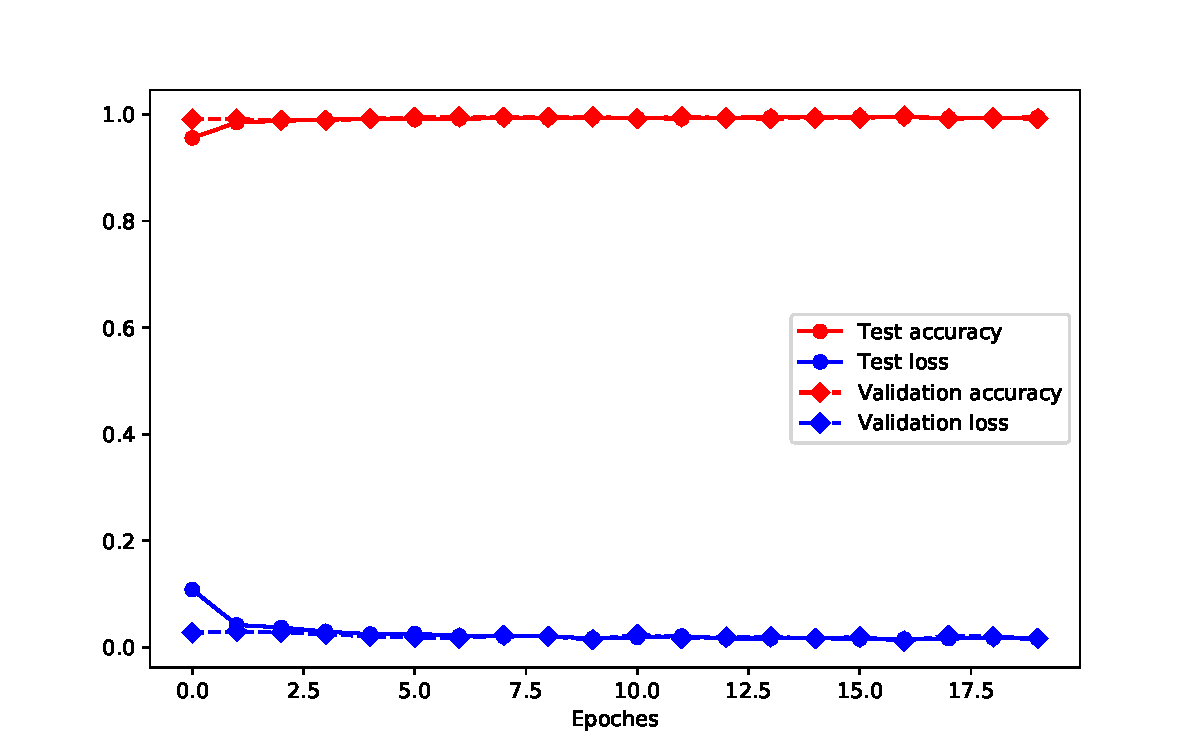
\includegraphics[width=0.85\linewidth]{Tex_proj/figure/training.pdf}
    \caption{Accuracy (top) and loss (bottom) of the Networks as function of the training epoch.}
    \label{fig:loss_train}
\end{figure}

\subsection{Face detector}
\texttt{OpenCV} does not provide metrics to evaluate the performances of ResNet-10 face detector; however we can still make some critical analysis on this model. We have that each object identified by the detector is associated to the \textit{confidence} parameter. We can set a minimum threshold for this parameter between 0 and 1, in order to filter weak face detections. A value near to 0 results in extracting ROIs even if no real faces are present, while if too high we can miss information. An example is shown in Figure~\ref{fig:test_2}, where we have a comparison with a confidence of 0.15 and 0.75. The higher value of 0.75 (bottom one) does not allow to catch all faces in the picture, while with 0.15 (top 2 images) we are able to extract more information.

\subsection{Predictions over real images}
\label{sec:images}
To better understand our models, some tests over images and videos are performed. This allows to better compare the two NN models trained for our classification task. Figure~\ref{fig:test_1} shows a quite simple scenario, where three people are walking in a public place with a straight on perspective. As we can see the face recognition is able to catch all the complete faces present in the pictures and we do not have a great distinction between the models. 

\begin{figure}[htp]
     \centering
     \begin{subfigure}[b]{0.4\textwidth}
         \centering
         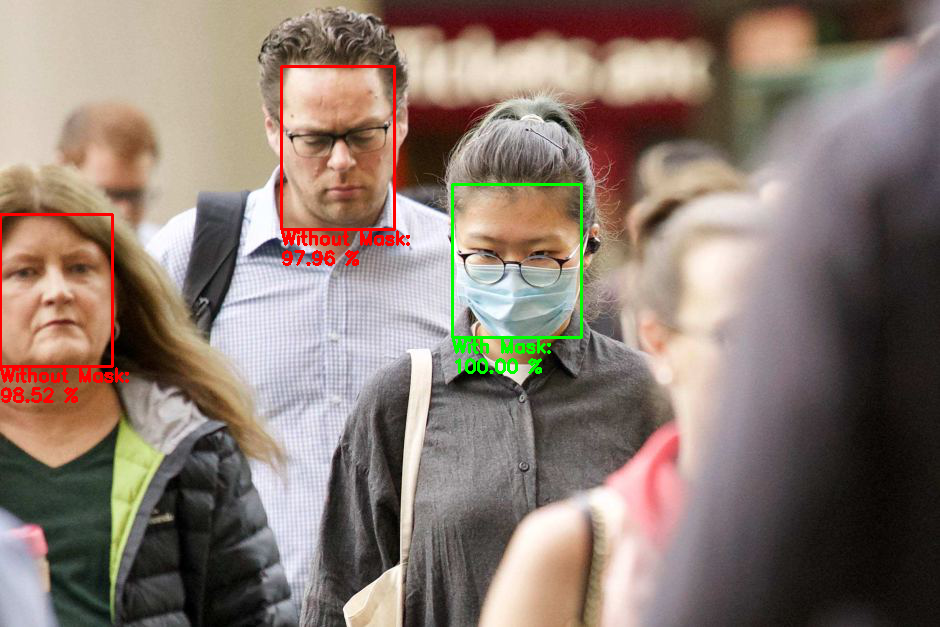
\includegraphics[width=0.90\linewidth]{Tex_proj/figure/test_1_pred_075_ConvNet.png}
         \caption{Convolutional Network and confidence at 0.75}
         \label{fig:conv_75_1}
     \end{subfigure}
     \begin{subfigure}[b]{0.4\textwidth}
         \centering
         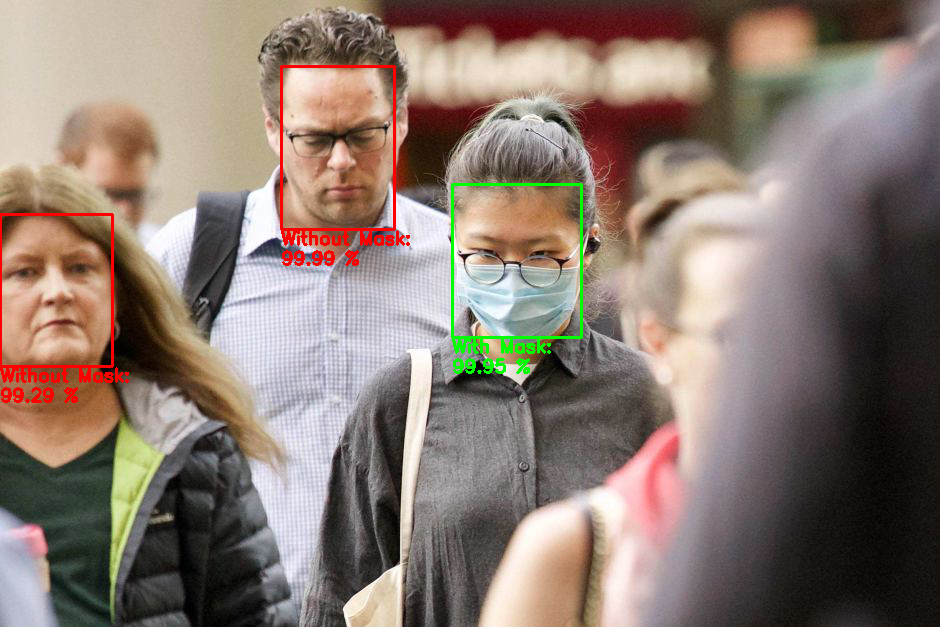
\includegraphics[width=0.90\linewidth]{Tex_proj/figure/test_1_pred_075_MobileNetV2.png}
         \caption{MobileNetV2 Network and confidence at 0.75}
         \label{fig:MN_75_1}
     \end{subfigure}
     \caption{}
     \label{fig:test_1}
\end{figure}

Figure~\ref{fig:test_2} is a more complex situation, which allows to notice some differences between the Networks and the importance of the confidence parameter. First of all we have to tune the confidence of the face detector to be able to catch all ROIs in the frame. In particular, we see some difficulties to detect people in the background or when faces are small and blurred and not looking straight on camera; in addition, also the fact of wearing a face mask makes the task more difficult: this is not surprising, since the face detector was trained over faces without masks. This is clearly noticeable in~\ref{fig:conv_75}.
Moreover, some misclassifications emerge (see~\ref{fig:mobnet_15}). This uncertainty with high probability is attributable to the train set, combined with the complexity of MobileNetworkV2. Furthermore, the simpler Convolutional architecture seems to act better when faces are blurred and in the background.

An additional evidence appears also in Figure~\ref{fig:test_3}, where the more complex model fails to correctly classify the woman on the left side.

%For example, as we will discuss in the future development, it is possible to have a wider training in which complex scenarios are labelled and the train can be more robust. Anyhow both the model don't have problem if we select standard faces in focus and quite centered but looking at the classification we have that the convolutional network seems to predict better the use of the mask. Another case in which the convolutional network seems to work better than the MobileNet is shown in figure \ref{fig:test_3}. As we can see the girl partially covered in the left side of the frame is misclassified by the complex network and our simple model is better in this type of prediction.

\begin{figure}[htp]
    \centering
    \begin{subfigure}[b]{0.5\textwidth}
        \centering
        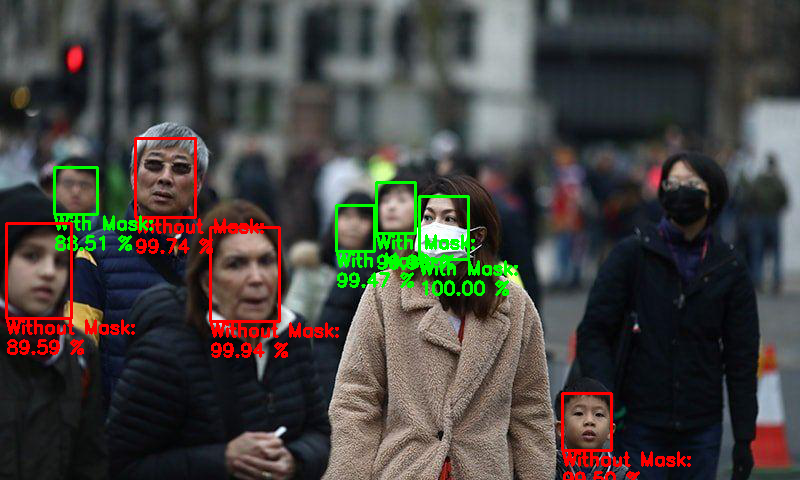
\includegraphics[width=0.80\linewidth]{Tex_proj/figure/test_2_pred_015_MobileNetV2.png}
        \caption{MobileNetV2 Network and confidence at 0.15}
        \label{fig:mobnet_15}
    \end{subfigure}
    \begin{subfigure}[b]{0.5\textwidth}
        \centering
        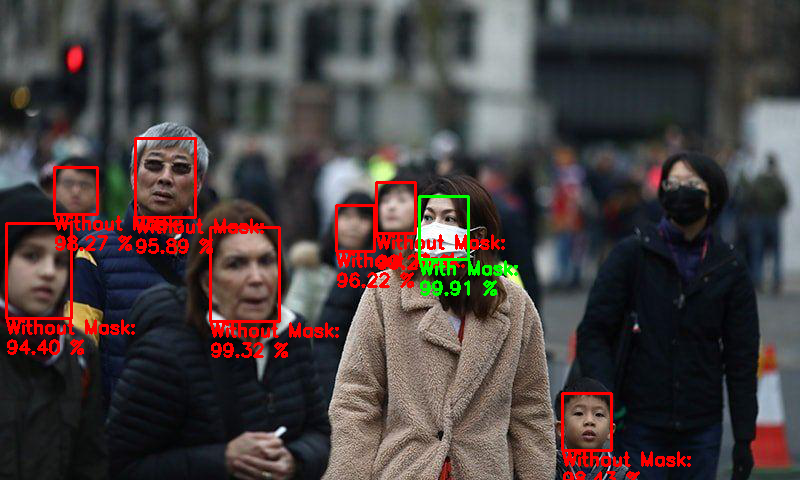
\includegraphics[width=0.80\linewidth]{Tex_proj/figure/test_2_pred_015_ConvNet.png}
        \caption{Convolutional Network and confidence at 0.15}
        \label{fig:conv_15}
    \end{subfigure}
    \begin{subfigure}[b]{0.5\textwidth}
        \centering
        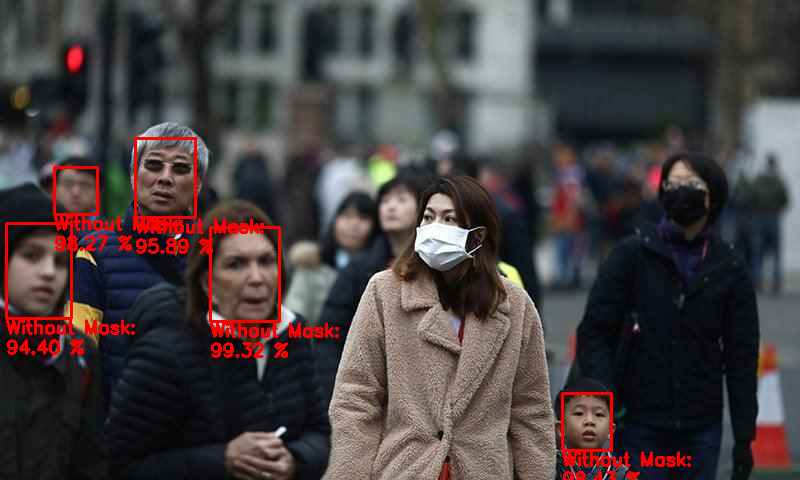
\includegraphics[width=0.80\linewidth]{Tex_proj/figure/test_2_pred_075_ConvNet.png}
        \caption{Convolutional Network and confidence at 0.75}
        \label{fig:conv_75}
    \end{subfigure}
    \caption{Comparison between the two Networks and different levels of confidence.}
    \label{fig:test_2}
\end{figure}

\begin{figure}[htp]
    \centering
    \begin{subfigure}[b]{0.4\textwidth}
        \centering
        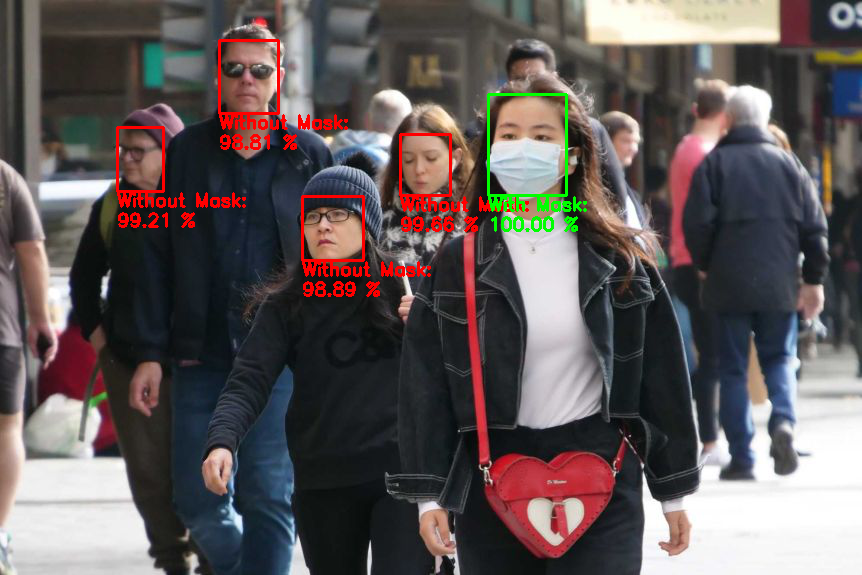
\includegraphics[width=0.90\linewidth]{Tex_proj/figure/test_3_pred_025_ConvNet.png}
        \caption{Convolutional Network and confidence at 0.25}
         \label{fig:conv_25_3}
    \end{subfigure}
    \begin{subfigure}[b]{0.4\textwidth}
        \centering
        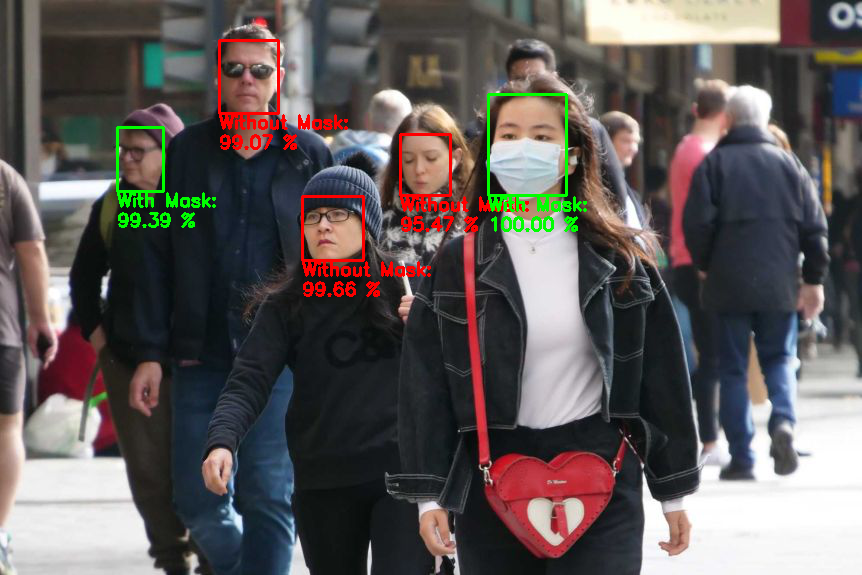
\includegraphics[width=0.90\linewidth]{Tex_proj/figure/test_3_pred_025_MobileNetV2.png}
        \caption{MobileNetV2 Network and confidence at 0.25}
        \label{fig:MN_25_3}
    \end{subfigure}
    \caption{}
    \label{fig:test_3}
\end{figure}

%The last pictures presented is figure \ref{fig:test_3} where again there is a mismatch between the classification make by the two networks. Again we have that the convolutional network seems to have a better confidence level.

In conclusion, the analyses over real images suggests that MobileNetV2 may have overfitted the data during the training phase, while the simpler model holds better generalization capabilities. More in detailed, greater differences happen when faces are not clear and in foreground, or when people are not looking straight into the camera.
As far as it concerns the face detector, the confidence threshold needs to be tune for each specific case, keeping in mind that we are trying to extract faces even if they are partially covered by the mask, so we need to allow low levels of the parameter.

\subsection{Video analysis}
\label{sec:video}
Predictions can also be made during video or real time streamings. This is a more challenging task, but it helps to gain a better knowledge of the models. 

One first study involves a video taken from \textit{TG3}, an Italian newscast, and a parallel analysis of MobileNetV2 and the Convolutional Network is proposed. Figure~\ref{fig:tg} show some snapshots taken from the video analysis. It sums up the three different major situations that in general happen:

\begin{itemize}
    \item If there are people looking in a frontal position with respect the the camera, both the models are able to get the right prediction (Picture~\ref{fig:tg_1});
    \item In~\ref{fig:tg_2} the face detector cannot extract ROIs if the face if largely covered, so no prediction is performed at all, sice nothing is passed to the classificator;
    \item The last case, the most probable in real life scenarios, applies to people looking away from the camera or standing quite far away from it. In this case, as shown in Figure~\ref{fig:tg_3}, the Convolutional Network seems to be more accurate and a lot more stable than the one based on MobileNetV2. 
\end{itemize}

The video analysis confirms the hypothesis raised in Section~\ref{sec:images}: the reliability of Convolutional Network is higher than the one of MobileNetV2 when applying the predictions to real life situations.

Also our streaming test endorse this assumption. In Figure~\ref{fig:stream} two snapshots are taken from a real time record from the PC webcam. MobileNetV2 is fooled by a subject having a beard: it is said to wear a mask even if it is not the case.

Another aspect that emerges from the videos is that MobileNetV2 changes rapidly the prediction and seems to be very unstable, while the Convolutional Network keeps the same response for a longer duration.

\begin{figure}[htp]
     \centering
     \begin{subfigure}[b]{0.5\textwidth}
         \centering
         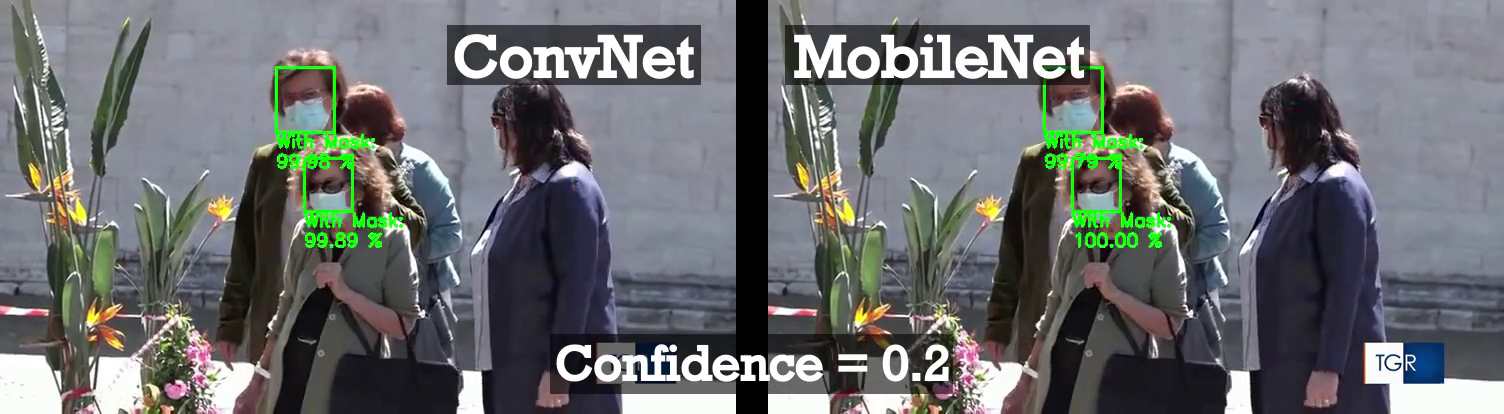
\includegraphics[width=0.9\linewidth]{Tex_proj/figure/tg3_screen_1.png}
         \caption{}
         \label{fig:tg_1}
     \end{subfigure}
     \begin{subfigure}[b]{0.5\textwidth}
         \centering
         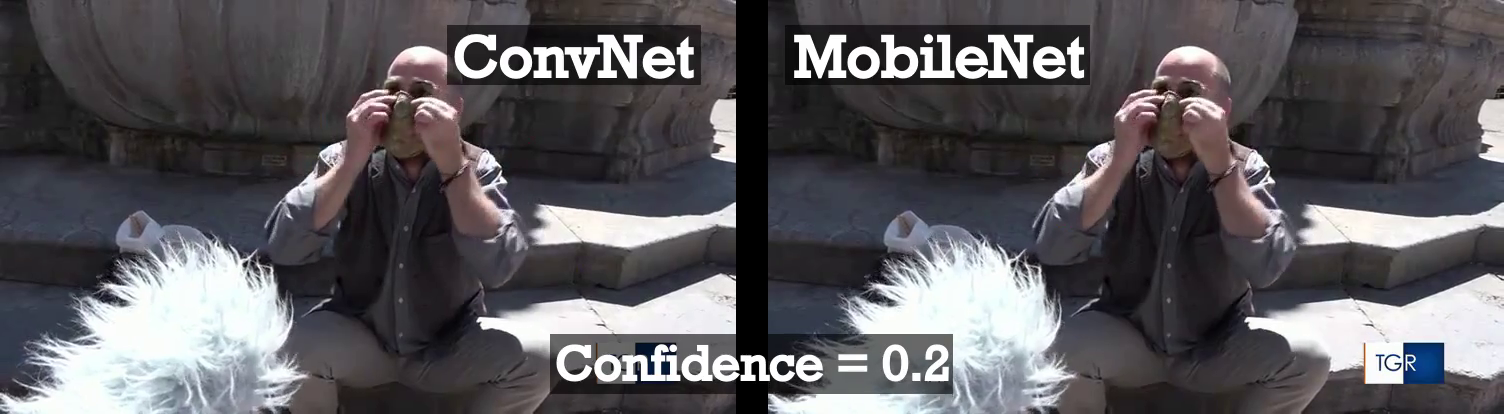
\includegraphics[width=0.9\linewidth]{Tex_proj/figure/tg3_screen_2.png}
         \caption{}
         \label{fig:tg_2}
     \end{subfigure}
     \begin{subfigure}[b]{0.5\textwidth}
         \centering
         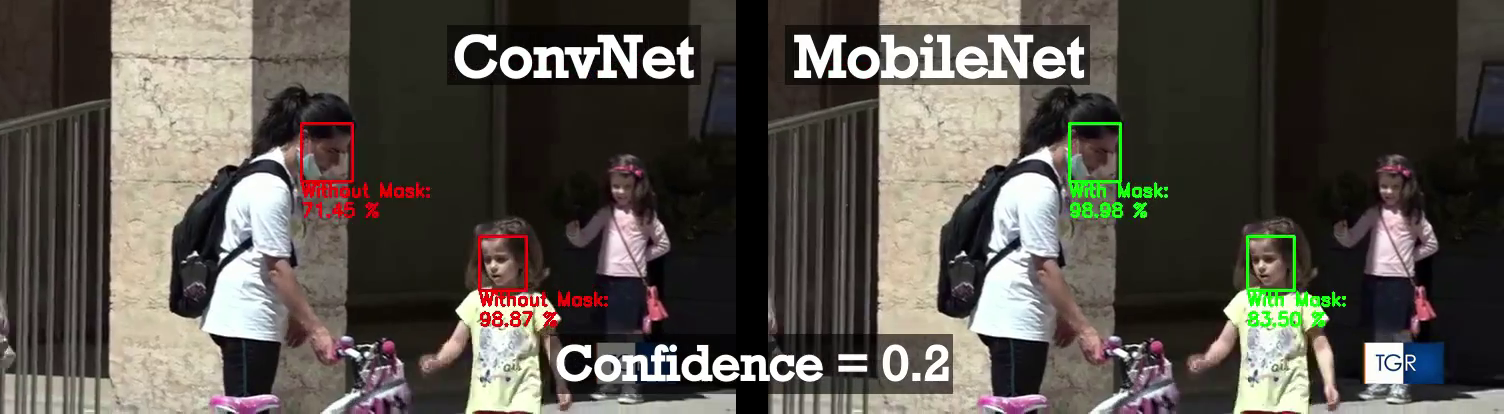
\includegraphics[width=0.9\linewidth]{Tex_proj/figure/tg3_screen_3.png}
         \caption{}
         \label{fig:tg_3}
     \end{subfigure}
     \caption{Snapshot taken from \textit{TG3} newscast video.}
     \label{fig:tg}
\end{figure}

\begin{figure}[htp]
     \centering
     \begin{subfigure}[b]{0.5\textwidth}
         \centering
         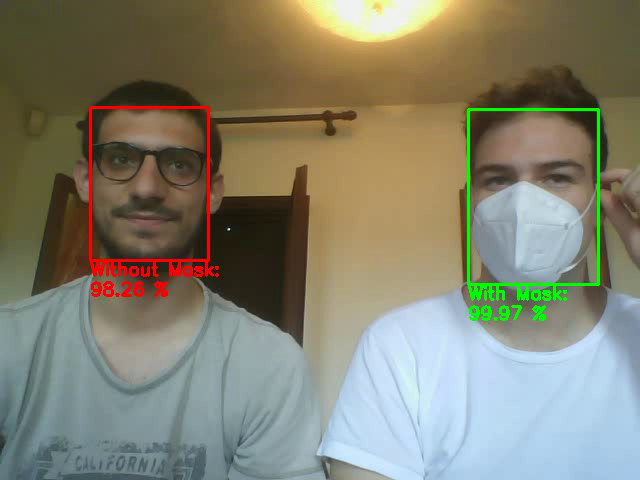
\includegraphics[width=0.80\linewidth]{Tex_proj/figure/stream_screen_Conv.png}
         \caption{Convolutional Network}
         \label{fig:stream_conv}
     \end{subfigure}
     \begin{subfigure}[b]{0.5\textwidth}
         \centering
         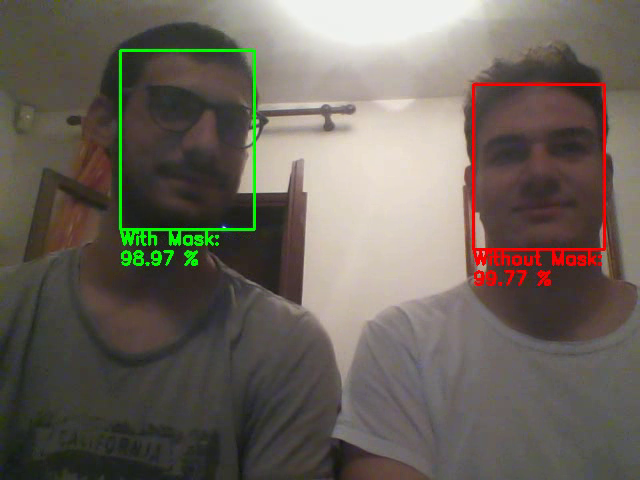
\includegraphics[width=0.80\linewidth]{Tex_proj/figure/strem_screen_MobNet.png}
         \caption{MobileNetV2}
         \label{fig:stream_MN}
     \end{subfigure}
     \caption{Snapshot taken from a real time streaming analysis.}
     \label{fig:stream}
\end{figure}

\section{Conclusions and future developments}
In this work a pipeline to detect whether people are wearing face masks is presented. First of all a face detector extract ROIs from images or videos, and then a NN makes the prediction. Two different predictors are tested, which feature architecture with dissimilar complexity. Experiments over real images and videos are performed to better understand the capabilities of the models.

Metrics extracted during the training of NNs leads to consider MobileNetV2 as the best candidate, with an accuracy of about 99\% against the 97\% of the Convolutional solution. Delving into the details, we discover that the test set that we use may be quite similar to the training one and so the results is a little bit biased (due to overfitting). Looking for more complex tests such as real pictures, videos and streaming, we discover that the Convolutional Network keeps a better stability in the previsions and produces more reliable forecasts;on the other hand, MobileNetV2 seems to flare during videos and it fails when the inputs are different from the ones given in the training phase (e.g. when faces are not straight to the camera, or are more blurred). The reason behind this behavior can be found in the complexity of the model itself. We have that MobileNetV2 is a very deep network that can be suitable for very complex tasks, but that can leads to overfitting when facing simpler scenarios like the one presented here. At the light of this discussion we can conclude that the Convolutional Network is to be preferred for our scope.

As far as it concerns the face detector, it needs to be pointed out that it is trained over a dataset that features faces without masks on them (even if the WIDER dataset collects situations with high degree of variability in scale, pose and occusion). This could lead to not catching ROIs when face masks are worn, since a great part is covered and hence it may not be detected; if this happens, no prediction is made, hence important information may be missed. To overcome this problem, the confidence parameter needs to be tune for each situation.

The bottleneck of our work is definitely the training set. Collecting a more heterogeneous series of images will surely boost the classification performances, allowing more complex models to be use effectively. For example, taking pictures and manually annotating the positions of the faces may be required to build data that features a vastness of different situations in terms of face positions, light, types of masks, \dots . 

However, in this case the bottleneck may only be shift towards the performances of the face detector. As already stated, it may have difficulties to make good detections if the face is covered. Hence, directly training the face detector to recognize not only faces, but also faces with masks can be the better solution. Also in this case a large dataset annotated by hand is required.

\section{Appendix}
\subsection{Graph}
\label{Grafo}
\begin{figure}[htp]
    \centering
    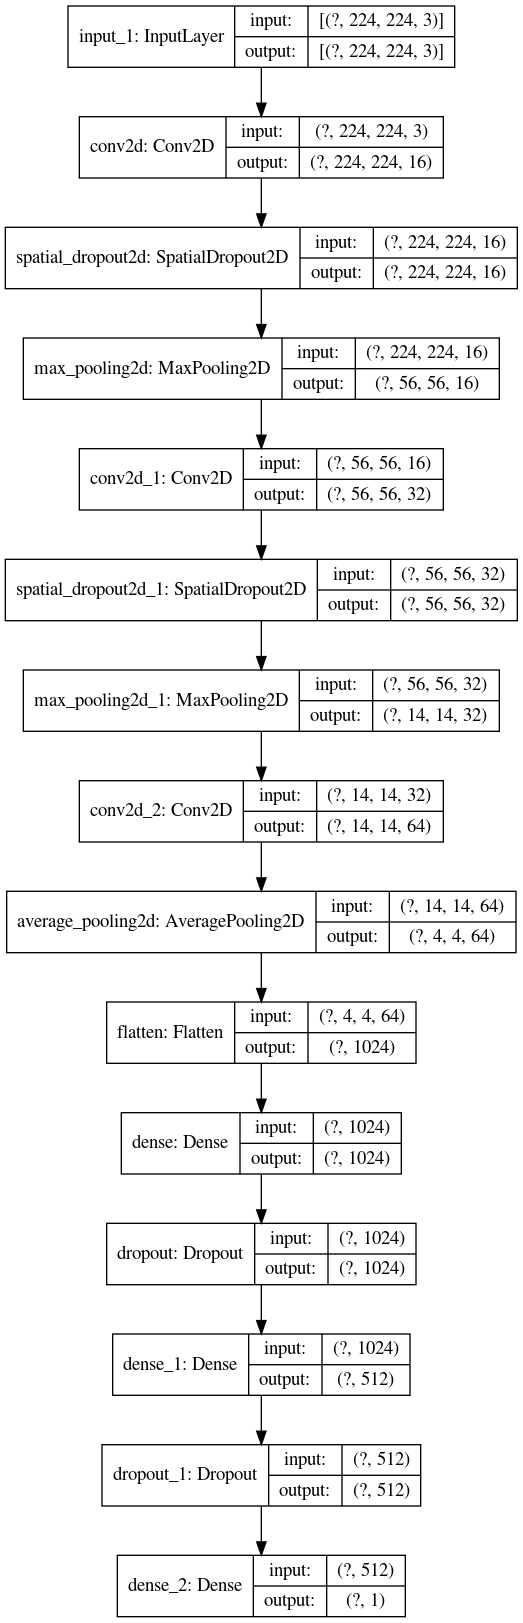
\includegraphics[width=0.50\linewidth]{Tex_proj/figure/model.png}
    \caption{Schematic representation of the Convolutional Neural Network.}
    \label{fig:grafo}
\end{figure}

\newpage

{\small
\bibliographystyle{ieee_fullname}
\bibliography{egbib}
}
\end{document}
